%\appendix
%\renewcommand{\thechapter}{B}

\chapter{An alternative choice for the source term in \chapref{chap:phmixlin}}
\label{ap:g1force}

The source term in \eqref{phmixlin:eq:g}, providing direct forcing of density perturbations, 
was a choice of convenience: it allowed us to compare directly the FDR
for the potential field $\phi$ in a kinetic system with the FDR for 
the Langevin equation \exref{phmixlin:eq:Langevin}. If, instead, one strives for 
a form of energy injection with a more transparent physical interpretation, 
it is natural to imagine it 
coming from a fluctuating electric field. This changes \eqref{phmixlin:eq:g} 
to the following:
\begin{align}
&\pd{g}{t} + v\,\pd{g}{z} 
+ v F_0 \pd{\phi}{z} = 
\chi_1(t) v F_0 + C[g] \;\!\!, \label{phmixlin:eq:g1force} \\
& \la \chi_1(t) \chi_1(t') \ra  = \eps \delta (t-t'), \nonumber
\end{align}
where $\chi_1(t)$ is the fluctuating parallel electric field, which we
model (again, for analytical convenience) as a Gaussian white noise. 

The new forcing injects fluctuations of momentum, rather than density. 
Indeed, in terms of Hermite moments, instead of \eqsand{phmixlin:eq:g0}{phmixlin:eq:g1}, 
we now have 
\begin{align} 
\label{phmixlin:eq:g0mom}
&\pd{g_0}{t} + \pd{}{z}\frac{g_1}{\sqrt{2}}  = 0,\\
\label{phmixlin:eq:g1mom}
&\pd{g_1}{t} + \pd{}{z}\lt(g_2 + \frac{1+\alpha}{\sqrt{2}}\,g_0\rt)  = \frac{\chi_1}{\sqrt{2}},
\end{align}
and \eqref{phmixlin:eq:gmeq} is unchanged. 
The field that is directly forced is $g_1 = \sqrt{2}\int \rmd v\,v g(v)$, which is 
proportional to the mean velocity associated with the perturbed distribution $g$. 
The new free-energy equation, an analog of \eqsand{phmixlin:eq:Wbalance}{phmixlin:eq:Wbal}, is 
\beq
\frac{\rmd W}{\rmd t} = \frac{\eps}{4} + \int\rmd v\,\frac{\la g C[g]\ra}{F_0}
= \frac{\eps}{4} - \nu \sum_{m=2}^\infty m\la g_m^2\ra.
\label{phmixlin:eq:Wbal1}
\eeq
This immediately gives us the universal Hermite spectrum and the FDR for the total 
free energy: we repeat the calculation in \secref{phmixlin:sec:flux} (which is unchanged 
because nothing has changed at high $m$'s) using the steady-state 
version of \eqref{phmixlin:eq:Wbal1} instead of \eqref{phmixlin:eq:Wbal_stst} to get 
\beq
A_k = \frac{\eps_k}{2\sqrt{2}|k|} 
\label{phmixlin:eq:Ak1}
\eeq
in the expression \exref{phmixlin:eq:Ccoll} for the Hermite spectrum. 
Therefore,   
\beq
\frac{1}{2}\sum_{m=1}^\infty \Cmk 
= \frac{\Gamma(1/3)}{4\cdot3^{2/3}}\frac{1}{\nu^{1/3}|k|^{2/3}}\,\eps_k
\label{phmixlin:eq:Wtot1}
\eeq
replaces \eqref{phmixlin:eq:Wtot} as the FDR for the total free energy. 
The only differences are in numerical prefactors and the $\alpha$ dependence, 
which has now disappeared. This is because in our previous 
forcing model, the source term injected
energy into $g_0$ (density fluctuations), which got scaled by the factor of $1+\alpha$ 
when passed on to $g_1$ (see \eqref{phmixlin:eq:g1}), 
whereas in the case we are considering now, the energy is injected directly into $g_1$, 
which is then phase mixed to higher $m$'s, without ever encountering any $\alpha$ dependence.  

\begin{figure}
\begin{center}
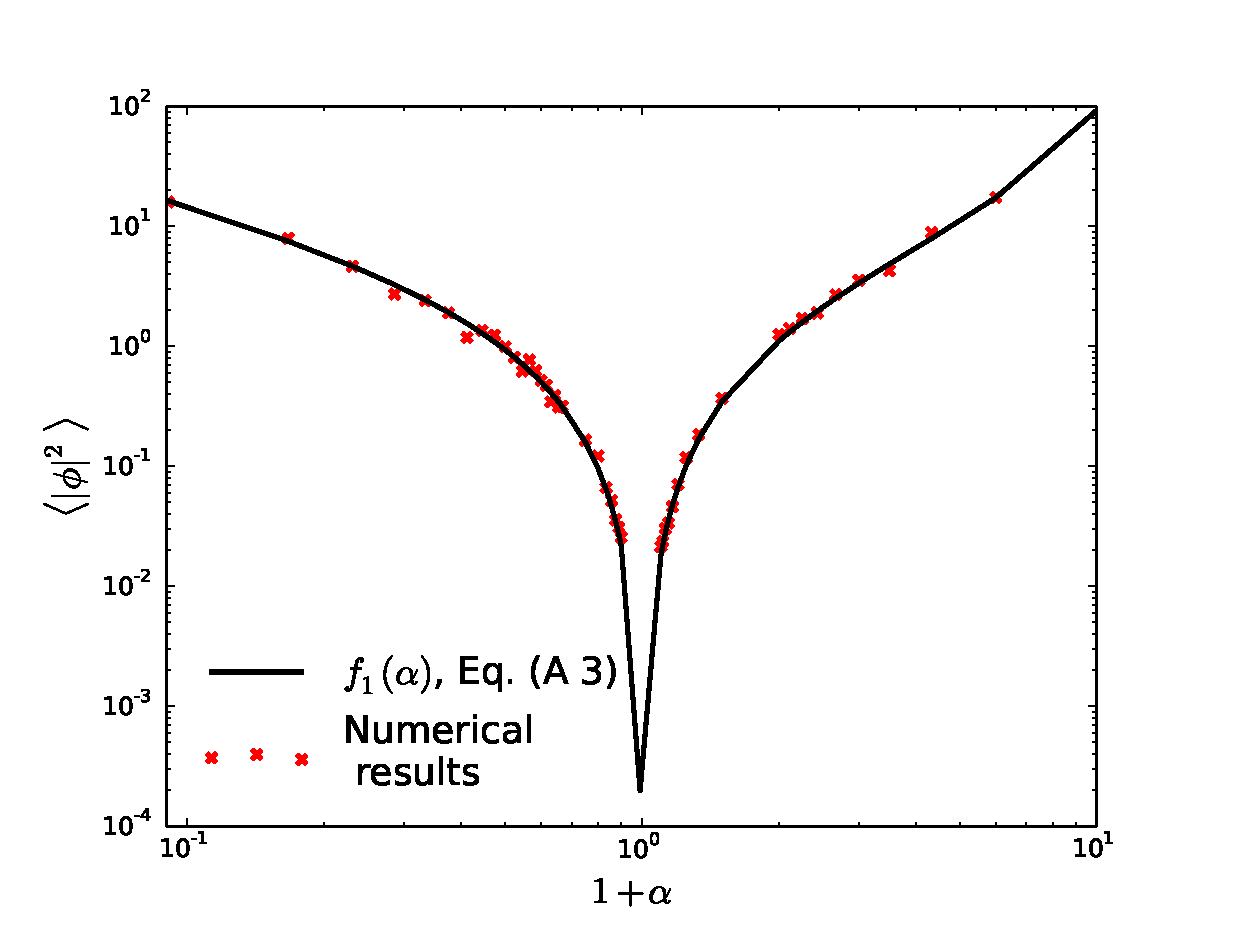
\includegraphics[width=10cm]{figs/phmixlin/phi2_g1.eps}
\caption{Normalized steady-state amplitude $2\pi|k|\la|\phi_k|^2\ra/\eps_k=f_1(\alpha)$ 
vs.\ $1+\alpha$ for the case of momentum forcing: 
the solid line is the analytical prediction $f_1(\alpha)$ (\eqref{phmixlin:eq:f1}), 
the crosses are computed from 
the long-time limit of $\la|\phi_k|^2\ra$ obtained via direct numerical 
solution of \eqref{phmixlin:eq:g1force}.}
\label{phmixlin:fig:f1}
\end{center}
\end{figure}

Let us also give here the results one obtains in the collisionless 
limit by backtracking to \eqref{phmixlin:eq:g1force} and solving for $g$ explicitly, 
as we did in \secsand{phmixlin:sec:FDR}{phmixlin:sec:FDR_Hermite}:
\beq
\gko = - \lt(\phiko + \frac{i\chikoone}{k}\rt)\frac{v F_0}{v - \omega/k}.
\label{phmixlin:eq:gko1}
\eeq
This gives
\begin{align}
\label{phmixlin:eq:phiko1}
\phiko &= - \frac{i\chikoone}{k}\frac{1 + \zeta Z(\zeta)}{D_\alpha(\zeta)},\\
\gmko &= - \frac{i\chikoone}{k}\frac{1}{\alpha}\frac{(-\sgn k)^m}{\sqrt{2^m m!}}
\frac{\zeta Z^{(m)}(\zeta)}{D_\alpha(\zeta)},\quad m\ge1,
\label{phmixlin:eq:gm1}
\end{align}
where $\zeta = \omega/|k|$ as usual. From the last formula, 
proceeding in the same manner as we did to get \eqref{phmixlin:eq:Cuniv}, we recover again
the Hermite spectrum: 
\begin{align}
\Cmk &= \frac{\eps_k}{2\pi|k|}\frac{1}{\alpha^2} 
\frac{1}{2^m m!}\int_{-\infty}^{+\infty}\rmd\zeta\lt|\frac{\zeta Z^{(m)}(\zeta)}{D_\alpha(\zeta)}\rt|^2\\
&\approx \lt[\frac{\eps_k}{\sqrt{2\pi}|k|}\frac{1}{\alpha^2}
\int_{-\infty}^{+\infty}\frac{\rmd\zeta\,\zeta^2 e^{-\zeta^2}}{|D_\alpha(\zeta)|^2}\rt]\frac{1}{\sqrt{m}}
=\frac{\eps_k}{2\sqrt{2 } |k|} \frac{1}{\sqrt{m}}. 
\label{phmixlin:eq:Cuniv1}
\end{align}
The latter expression was obtained in the limit of $m\gg1$ (see \secref{phmixlin:sec:spectrum}) 
and is the same result as \eqref{phmixlin:eq:Ak1}. The integral is already familiar from \eqref{phmixlin:eq:Cminus}. 
For completeness, the ``$-$''-mode spectrum \exref{phmixlin:eq:Cminus} becomes 
\beq
\Cmk^- \approx \lt[\frac{\eps_k}{8\sqrt{2\pi}|k|}\frac{1}{\alpha^2}
\int_{-\infty}^{+\infty}\frac{\rmd\zeta\,\zeta^4
e^{-\zeta^2}}{|D_\alpha(\zeta)|^2}\rt]\frac{1}{m^{3/2}} 
 = \frac{\eps_k (3+\alpha)}{32 \sqrt{2} |k|} \frac{1}{m^{3/2}}. 
\label{phmixlin:eq:Cminus1}
\eeq
The integral was done by Kramers--Kroning relations
for the function $h(\zeta) = \zeta^4/D_\alpha(\zeta) - \alpha\zeta^4 - \alpha^2\zeta^2/2 
- \alpha^2(3+\alpha)/4$. While again numerical prefactors and $\alpha$ dependence 
are different, none of the substantive arguments in \secref{phmixlin:sec:cont} are affected. 

Finally, from \eqref{phmixlin:eq:phiko1}, 
proceeding in the same manner as in \secref{phmixlin:sec:FDR}, we obtain the FDR 
relation for the mean square fluctuation amplitude of the potential:
\beq
\la |\phi_k|^2 \ra = \frac{\eps_k }{2 \pi |k|} f_1(\alpha), \quad
f_1(\alpha) = \int_{-\infty}^{+\infty}\rmd\zeta
\lt|\frac{1 + \zeta Z(\zeta)}{D_\alpha(\zeta)}\rt|^2,
\label{phmixlin:eq:f1}
\eeq
which is the new version of \eqref{phmixlin:eq:f}. 
The function $f_1(\alpha)$ is plotted in \figref{phmixlin:fig:f1}, along with
the results of the direct numerical solution of \eqref{phmixlin:eq:g1force}.
While formally it is a different function than $f(\alpha)$, 
it exhibits very similar behavior (see \figref{phmixlin:fig:f}).  
Its asymptotics are (see \secsand{phmixlin:sec:small}{phmixlin:sec:large})
\begin{align}
\label{phmixlin:eq:FDR_small1}
\alpha\to-1: & \quad
f_1(\alpha) \approx \frac{|k|}{\gamma_L}
\quad\Rightarrow\quad
\la|\phi_k|^2\ra\approx \frac{\eps_k}{2\pi \gamma_L},\\
\alpha\to\infty: & \quad
f_1(\alpha) \approx \frac{\pi\alpha |k|}{4 \gamma_L}
\quad\Rightarrow\quad
\la|\phi_k|^2\ra\approx \frac{\alpha \eps_k}{8 \gamma_L}.
\label{phmixlin:eq:FDR_large1}
\end{align}
Whereas in both limits there is still an inverse relationship between 
the mean square fluctuation amplitude and the Landau damping rate 
$\gamma_L$, the numerical coefficients are not easily interpretable 
in terms of any simple ``fluid'' Langevin models for $\phi$---not a
surprising outcome as, already examining \eqsand{phmixlin:eq:g0mom}{phmixlin:eq:g1mom}, 
we might have observed that they do not map on any obvious 
Langevin-like equation for $\phi=\alpha g_0$.
%\footnote{The closest 
%to a Langevin-like form one gets is by rewriting these equations 
%in terms of two ``modes'' $u_\pm = g_1 \pm \sqrt{1+\alpha}\, g_0$, which satisfy 
%$\dd_t u_\pm \pm \omega_0 \dd_z u_\pm + \dd_z g_2 = \chi_1/\sqrt{2}$, 
%where $\omega_0=\sqrt{(1+\alpha)/2}$. This system has a source, a real frequency 
%$\omega_0$, and a damping that enters via the phase-mixing term $\dd_z g_2$.
%This damping is not, however, representable as $\gamma_L u_\pm$.} 
The elementary Landau-fluid closure that in \secref{phmixlin:sec:LF} neatly 
mapped the $\alpha\to-1$ limit onto a ``fluid'' Langevin equation, 
when reworked for the case of the momentum forcing, gives
\beq
\pd{\phi_k}{t} + \gamma_L \phi_k = \frac{\sgn k}{\sqrt{\pi}}\chi_{1,k}.
\label{phmixlin:eq:LF1}
\eeq
Thus, a Langevin equation still, but with an order-unity adjusted noise term.  




